\documentclass[10pt,conference,compsocconf]{IEEEtran}

\usepackage{hyperref}
\usepackage{graphicx}	% For figure environment
\usepackage{subfigure}
\usepackage{titling} % Customizing the title section
\usepackage{dblfloatfix}    % To enable figures at the bottom of page
\usepackage{kantlipsum}     % for random text
\usepackage{todonotes}
\usepackage[margin=0.9in]{geometry}
\usepackage{multirow}
\usepackage[margin=0.9in]{geometry}
\usepackage[english]{babel}
\usepackage{dsfont}
\usepackage[font={small,it}]{caption}
\usepackage{array}
\usepackage{siunitx} 
\usepackage{float}
\restylefloat{table}

\begin{document}
	
\pretitle{\begin{center}\Huge\bfseries} % Article title formatting
\posttitle{\end{center}} % Article title closing formatting
\title{Deep Learning - Project 1}

\author{
	% Your name
	\textsc{Niccol\`{o} Sacchi, Succa Riccardo \& Marco Zoveralli}
	\normalsize{} \\
	% Your supervisors
	%\textsc{Group:}
	%\normalsize{RoadSegmentationFault}\\
	% Your institution
	\normalsize \'{E}cole polytechnique f\'{e}d\'{e}rale de Lausanne
}

\maketitle

\begin{abstract}
  The goal of this project is to train and test a predictor of finger movements from Electroencephalography (EEG) recordings. We decided to implement several solutions, starting from simple baseline models and then escalating to complex deep neural networks. 
\end{abstract}

\section{Introduction}
This project consists in a two-class classification problem to predict incoming finger movements 130ms before key-press. The electrical pulse that generates the finger movement starts a fraction of second before the actual movement, giving us clues on which hand the subject is going to move through an EEG analysis.

The following sections give an overview of the techniques that were tried in order to construct the predictors. Section~\ref{sec:data-analysis} briefly describes the dataset of EEG recordings and the experiment that was performed to obtain them. Section~\ref{sec:baseline} proposes a first approach to the problem by using a series of simple classification models (baselines). Section~\ref{sec:deep} goes to more complex solutions exploiting Convolutional Neural Networks and Residual Neural Networks. Section~\ref{sec:results} compares the results obtained with the different models.

\section{Dataset}
\label{sec:data-analysis}
The dataset was provided by Fraunhofer-FIRST, Intelligent Data Analysis Group (Klaus-Robert M\"uller), and Freie Universit\"at Berlin, Department of Neurology, Neurophysics Group. It was first given in the "BCI competition II" (May 2003) with a sample of 416 epochs, divided in 316 train records (labeled) and 100 test records (unlabeled).
The experiment performed to create the dataset consisted in examining a normal subject sitting on a chair in a relaxed position, while he was typing on a computer keyboard in a self-chosen order. Three sessions of six minutes were taken, all conducted in the same day with a small break in-between and with an average typing speed of 1 key/second. The EEG records were made by using 28 electrodes to monitor the brain electrical activity. They measured a time slot of 500ms, ending 130ms before the key-press, with a sample frequency of 1000Hz but also provided in a downsampled version of 100Hz. In our project we used the records sampled at 100Hz, where each record is represented as a 28 (electrode's measurements) x 50 (time frames) matrix. 
An example of a record with the respective label is shown in figure~\ref{fig:Sample}.

\begin{center}
	\captionsetup{type=figure}
	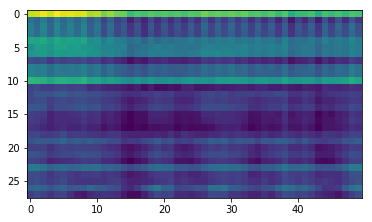
\includegraphics[width=0.5\textwidth]{img/sample.png}
	\caption {Sample from the dataset with label 1 (right movement)}
	\label{fig:Sample}
\end{center}


\section{Baseline Models}
\label{sec:baseline}
All the baseline models were tested with cross-validation and tuned with a grid search over some parameters. The input samples have been simply flattened to comply with the shape accepted by these baselines. Here we list some of the tried models, imported from the \textit{sklearn} library:
\begin{itemize}
\item \textit{Logistic Regression}. Tuned parameter: regularization. 
\item \textit{Random Forest Classifier}. Tuned parameter: max depth of the trees.
\item \textit{K-Nearest Neighbors}. Tuned parameter: K. Moreover, before training this model, we normalized the input and applied a PCA to reduce the dimensions (we kept the 95\% of the signal energy).
\end{itemize}

Table \ref{tab:baselineres} shows that none of the baselines is really able to provide a proper solution to this problem. In the next section we show the improvements that were obtained through the adoption of our own models and the methodology behind their construction. However, surprisingly, The Logistic regression model achieves good accuracy, despite the fact that it is much simpler than other models we tried.

\begin{table}[H]
\caption{Test accuracies obtained on tuned baselines.}
\label{tab:baselineres}
\centering
\begin{tabular}{ | c | c | }
\hline
Baseline & Test Accuracy \\
\hline
LogisticRegression & $70\%$ \\
\hline
Random Forest Classifier & $58\%$ \\
\hline
K-NN & $54\%$ \\
\hline
\end{tabular}
\end{table}

\section{Deep Neural Networks}
\label{sec:deep}
%We designed different models, starting from a simple Convolutional Neural Network and then tuning the parameters to reach more complex solutions.\\
%The increasing complexity of these models allowed us to get better perfomances on the test set, at the price of more time and resources needed.\\
Our methodology was based, at first, on building networks inspired to the concepts introduced during the lectures and then, we focused on tuning these models with the goal of improving the results.

%\subsection{Cross-validation}
One fundamental aspect of our approach is to perform a \textit{grid search} over a set of parameters of the network and using a \textit{cross-validation} for each combination. The cross-validation technique consists, as first step, in splitting the available train dataset in k equal parts. Then, k-1 of these sets are used to train the model and 1 is used as a validation dataset. This process is repeated k times: at each iteration, a different part is considered as validation dataset and the remaining k-1 parts are taken as training dataset. This procedure must be repeated for a set of possible values that this parameter can assume. Finally, the parameter value that lead to the best average validation score is considered as best one.

Two further issues must be taken into account. First, there are a lot of parameters that influence the score. We took into account some of the most relevant: the number of layers, the regularization terms, the type of activation functions (i.e. ReLU, Tanh, ELU) and optimizers (i.e. Adam, Adamax, Adadelta), and the number of hidden units in the last fully connected layer. However, other relevant parameters are not considered during this optimization phase. For instance, we are not iterating through the number of filters, the filter dimensions and the learning rate. Second, getting the optimal combination of parameters implies enumerating all the possible combinations of all the parameters. This results in \textit{exponential complexity} and, after some tries, we observed that this is unfeasible for our available computational resources. Therefore, we adopted an approximation of the grid search method, which consisted in a greedy approach where we selected the optimal parameters singularly and sequentially. Although this does not provide an optimal solution, it allows to keep the algorithm complexity at an acceptable level (linear). With this approach, we have to carefully choose the parameter's order. First, we search over the parameters that mostly influence the model structure, in particular the number of layers, the number of hidden units and the activation function. Then, the grid search moves to the optimizer's parameters (optimization function and weight decay) and the dropout parameter. After all the parameters are defined, we decided to perform again a search over the number of layers, as it is expected to have high influence on the performance of the model and its best value may change after the other parameters are set.
The table \ref{tab:netarch} summarizes the grid search results for all the networks.

\subsection{CNN: 2D Convolutional Layers}
The first model that we tried is a 2D Convolutional Neural Network. After a grid search on the parameters, we obtained the structure in figure \ref{fig:Conv2D}: it consists in 5 convolutional layers, ReLU as activation function and Adadelta as optimizer.

\begin{center}
	\captionsetup{type=figure}
	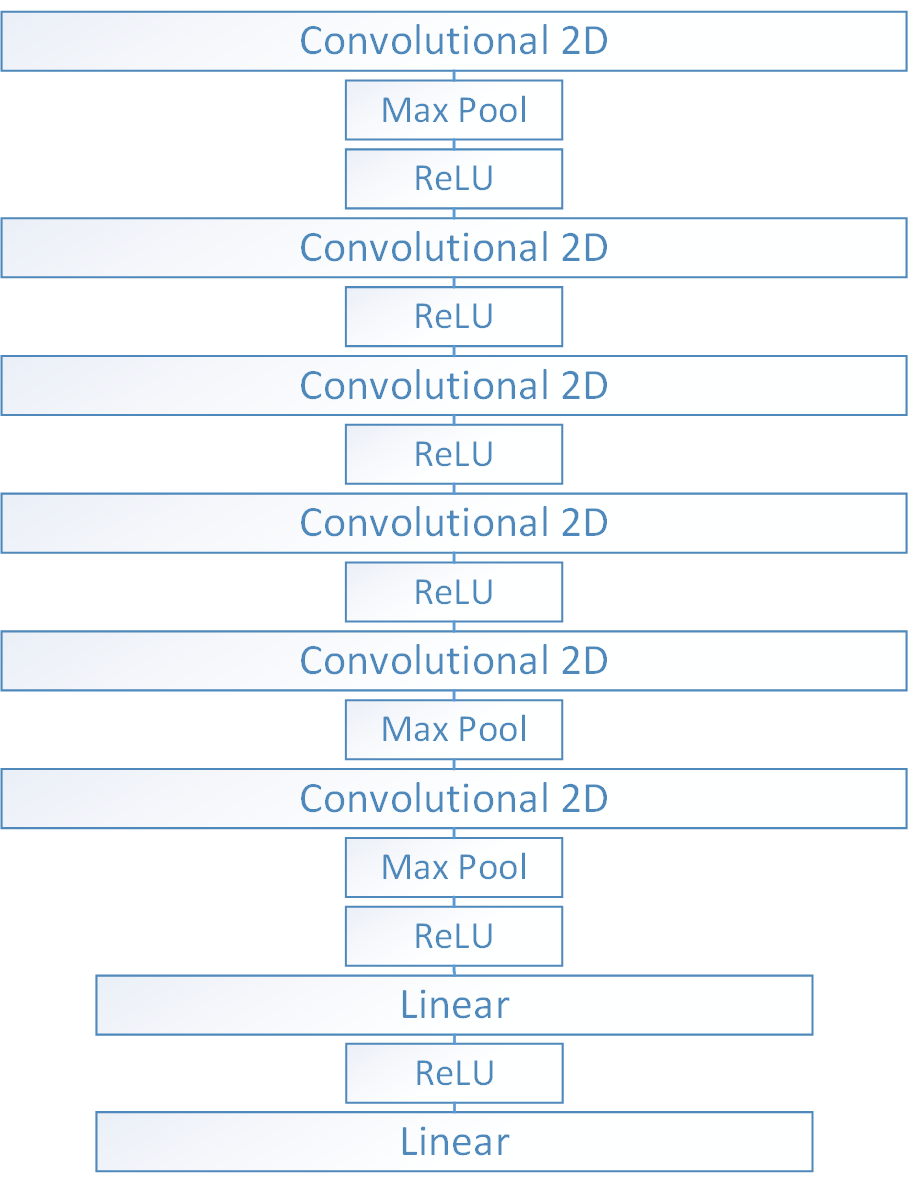
\includegraphics[width=0.35\textwidth]{img/Conv2D.png}
	\caption {2D Convolutional Neural Network}
	\label{fig:Conv2D}
\end{center}

\begin{table*}
	\caption{Network Architectures}
	\label{tab:netarch}
	\begin{tabular}{ | p{3cm} | p{2cm} | p{2cm} | p{2cm} | p{2cm} | p{2cm} | p{2cm} | }
		\hline
		Network & \#Additional Layers & \#Hidden Units & Optimizer & Activation Function & Regularization term & Dropout\\
		\hline
		A: 2D CNN
		& 3 & 40 & Adadelta & ReLU & 0.0 & 0.0 \\
		\hline
		B: 1D CNN
		& 4 & 40 & Adamax & ELU & 0.0025 & 0.1 \\
		\hline
		B: 1D CNN + Batch Norm
		& 5 & 160 & Adamax & ELU & 0.0025 & 0.3 \\
		\hline
		B: 1D CNN + Batch Norm + Dilation
		& 1 & 40 & Adamax & ELU & 0.135 & 0.1 \\
		\hline
		C:	Residual 1D CNN
		& 6 & 120 & Adamax & Tanh & 0.007 & 0.2 \\
		\hline
	\end{tabular}
\end{table*}

This network uses 2D convolutional layers, because at first it seemed natural to treat the provided dataset as a set of images. Therefore, the network was trying to find patterns between close pixels, by applying 2D filters over the input. This approach makes sense if there is a spatial relationship among the features. In our case, as mentioned in \ref{sec:data-analysis}, the input sample consists of 28 signals (EEG channels) captured over different time frames. Since the positions of the channels are not known, we cannot assume any spatial relationship between them. Therefore, applying a 2D filter over this dataset might try to find patterns between channels that are not spatially correlated. Consequently, we decided to process them all together by applying a 1D filter instead of a 2D. 


\subsection{CNN: 1D Convolutional Layers}
For the 1D CNN, we started with a simple structure and then we increased the complexity by adding more modules. In the first CNN, we only included dropout layers. Then, we used Batch Normalization, which provides significant improvements in terms of test accuracy and stability of the training. It focuses on performing normalization at each layer, and one of the main benefits is the mitigation of the change of the input distribution that may occur across the network layers. Finally, we added a dilation in the convolutional layers, hoping that increasing the receptive view of the filters could bring an improvement. Among these three variants, the best results were obtained by the 1D CNN with Batch Normalization (see Section \ref{sec:results} for the details). The structure is shown in figure \ref{fig:Conv1D}.

\begin{center}
	\captionsetup{type=figure}
	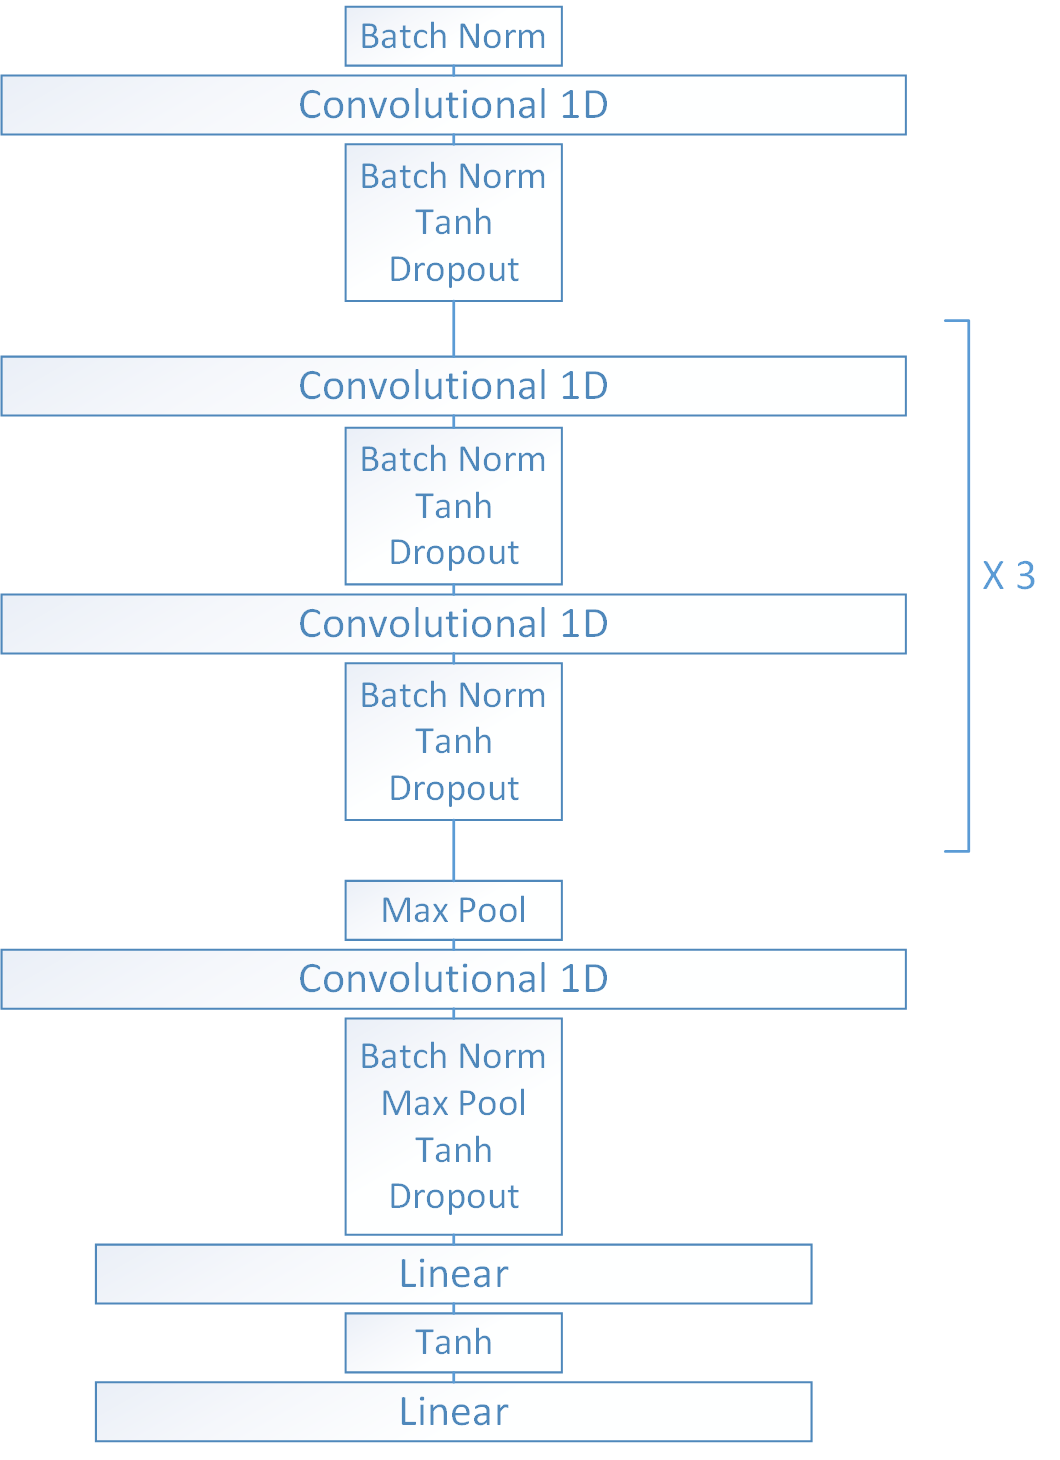
\includegraphics[width=0.37\textwidth]{img/Conv1DBatchNorm.png}
	\caption {1D Convolutional Neural Network with Batch Normalization}
	\label{fig:Conv1D}
\end{center}

One remark that concerns all the networks that involve batch normalization: although some sources\footnote{Batch Normalization: Accelerating Deep Network Training by Reducing Internal Covariate Shift - Sergey Ioffe, Christian Szegedy} claim that batch normalization makes the dropout advatanges negligible, we decided to try to tune both parameters during the grid search in any case.


\subsection{Residual 1D CNN}
This model consists in a series of aggregated residual blocks. Each residual block is made of a predefined number of convolutional layers, but the peculiarity of the block is that the input is also propagated directly to the output. Then, a group of residual blocks (two by default) are put together to construct an aggregated block. The grid search for the model iterated on the number of aggregated blocks connected sequentially. Figure \ref{fig:Residual} shows the final structure.

%A Residual CNN contains convolutional layers, linear layers, and a set of residual layers. Residual layers consist in having a block of convolutional layers (replicated a certain amount of times) whose output (at the end of the block) is influenced by the input of the block too. Our model accepts an arbitrary number of such blocks (each block has three convolutional layers), but by default there are two of them.

\begin{center}
	\captionsetup{type=figure}
	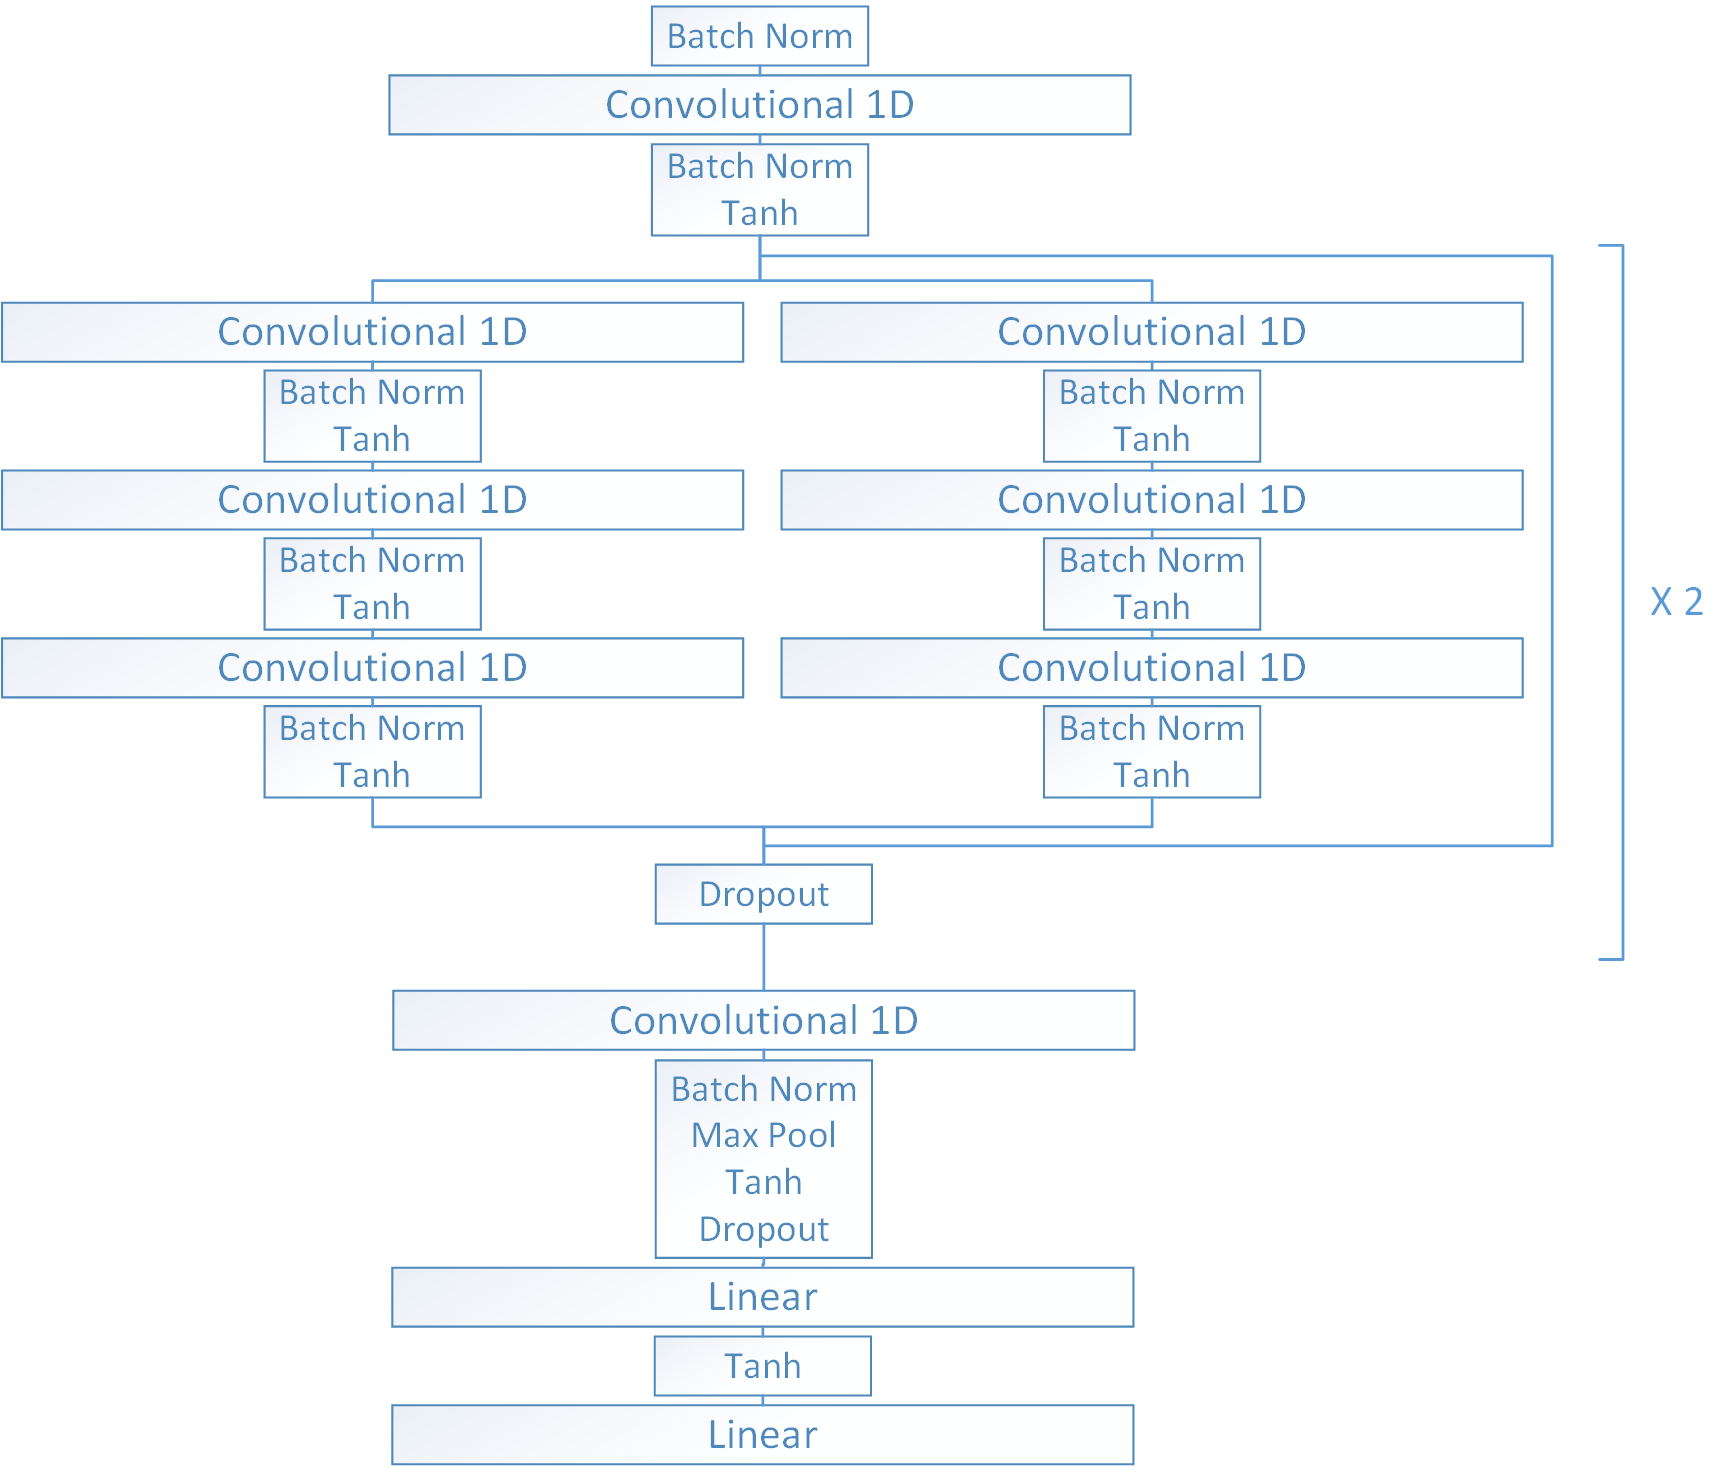
\includegraphics[width=0.5\textwidth]{img/Residual1D.png}
	\caption {1D Residual Neural Network}
	\label{fig:Residual}
\end{center}

Even if residual CNN are mainly used in the field of computer vision, we decided to try this type of network with our dataset. As we will show in section \ref{sec:results}, although the complexity of the model is much higher than the previous 1D and 2D CNN, the results did not improve in equal measure.

\section{Results}
\label{sec:results}
We now present the results of the networks that we described in the previous section. After each model has been tuned tuned with a grid search over the parameters, we tested them with a cross-validation on the train set and with a final evaluation over the test set. Figure \ref{fig:CrossVal} shows the results of the cross-validation.

\begin{center}
	\captionsetup{type=figure}
	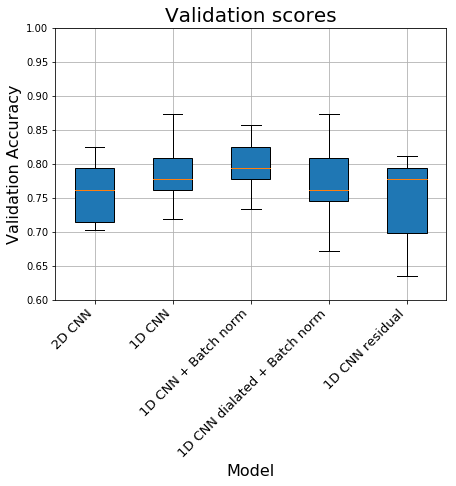
\includegraphics[width=0.45\textwidth]{img/CrossVal.png}
	\caption {Result of the Cross Validation on the train set.}
	\label{fig:CrossVal}
\end{center}

On the test set, the results are the following:

\begin{center}
	\captionsetup{type=figure}
	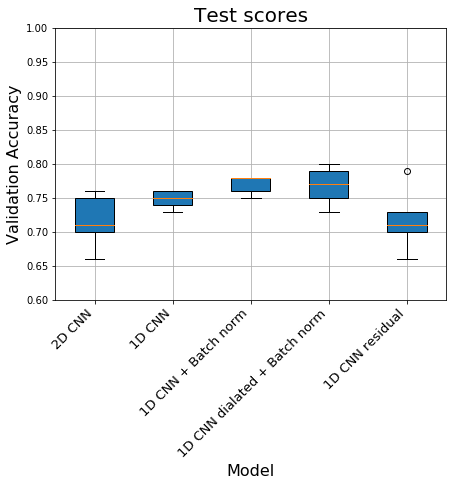
\includegraphics[width=0.45\textwidth]{img/TestVal.png}
	\caption {Result of several training on the test set.}
	\label{fig:CrossVal}
\end{center}

\begin{table}[H]
	\caption{Accuracy Table}
	\label{tab:accuracy}
	\begin{tabular}{ | p{3cm} |  p{2cm} |  p{2.1cm} | }
		\hline
		Network & Cross Validation Accuracy & Test Accuracy\\
		\hline
		2D CNN
		& $76.0\% \: \pm \: 4.6\%$ & $71.6\% \: \pm \: 3.6\%$ \\
		\hline
		1D CNN
		& $78.8\% \: \pm \: 5.2\%$ & $74.8\% \: \pm \: 1.2\%$\\
		\hline
		1D CNN + Batch Norm
		& $79.8\% \: \pm \: 4.2\%$ & $77.0\% \: \pm \: 1.3\%$\\
		\hline
		1D CNN + Dial + Batch Norm
		& $77.2\% \: \pm \: 6.7\%$ & $76.8\% \: \pm \: 2.6\%$\\
		\hline
		1D CNN Residual
		& $74.3\% \: \pm \: 6.7\%$ & $71.8\% \: \pm \: 4.3\%$\\
		\hline
	\end{tabular}
\end{table}

We noticed that the results on the test set are quite unstable. This is due to the noise and the size of the dataset. These limitations affect the training in the sense that it is hard for a model to always converge to the same solution  and identify meaningful patterns. Moreover, since the test set is very small (only 100 samples), mispredictions can substantially affect the test score which hardly reflect the actual performance of the model. We tried to overcome this problem by training several time the same model and providing the means and standard deviation of the obtained test scores. In order to avoid overfitting, we also choose an optimal number of epochs, i.e. the number for which the validation loss is minimized. Then this number of epochs has then been used for the test. From the boxplots above, the 1D Convolutional with Batch Normalization seems to be the best one, with an accuracy mean slightly better than the others and with lower standard deviation. For this model we also show how the loss decreases with the three different optimizers that we tried in our grid search which automatically selected the Adamax optimizer:

\begin{center}
	\captionsetup{type=figure}
	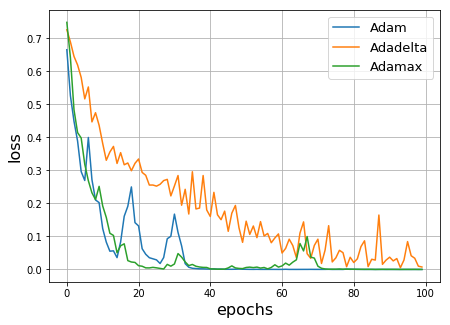
\includegraphics[width=0.45\textwidth]{img/optimizationAdam.png}
	\caption {Loss function for different optimizers}
	\label{fig:CrossVal}
\end{center}
We can notice that the loss function decreases faster and with more stability when using the Adamax optimizer.

\section{Conclusion}
\label{sec:conclusion}
The results that we obtained are partially satisfying. On one hand, the test accuracy is not excellent. The reasons can be found in the limited size of the train and test set and in the fact that no preprocessing was performed. Understanding the nature of the input signal was beyond the goal of this project, but an accurate analysis on the EEG dataset could have led to better results.

Still, the methodology that we followed allowed us to improve the models at each step and compare them in order to select the expected best one. The limitation of the computational power forced us to apply an approximation of the grid search technique. It can be argued that an extensive search on the parameters could have given an higher accuracy for all the models.


\end{document}
